
\section{Algoritmos de predicción} % (fold)
\label{sec:algoritmos_de_prediccion}

\subsection{Regresión Logística} % (fold)
\label{sub:regresion_logistica}


% subsection explorando_el_set_de_datos (end)

\subsection{Deduciendo features} % (fold)
\label{sub:deduciendo_features}

Como parte de preprocesamiento, necesitaremos deducir cuales son los datos importantes para nosotros, es decir cuales son los datos que van a ayudar a que nuestro algoritmo aprenda más eficientemente y prediga mejor. Esos datos se pueden encontrar directamente en el set de datos tal como está o pueden necesitar algún procesamiento previo. Algunos inclusive pueden ser combinación de varios datos de una fila.

Los únicos datos discretos, que sirven directamente son el distrito y el día de semana. La fecha tal como viene no tiene valor: cada crímen tiene una fecha única y lo más probable es que en el set de prueba tampoco se repita. Necesitamos procesar esa fecha primero.

\begin{figure}[H]
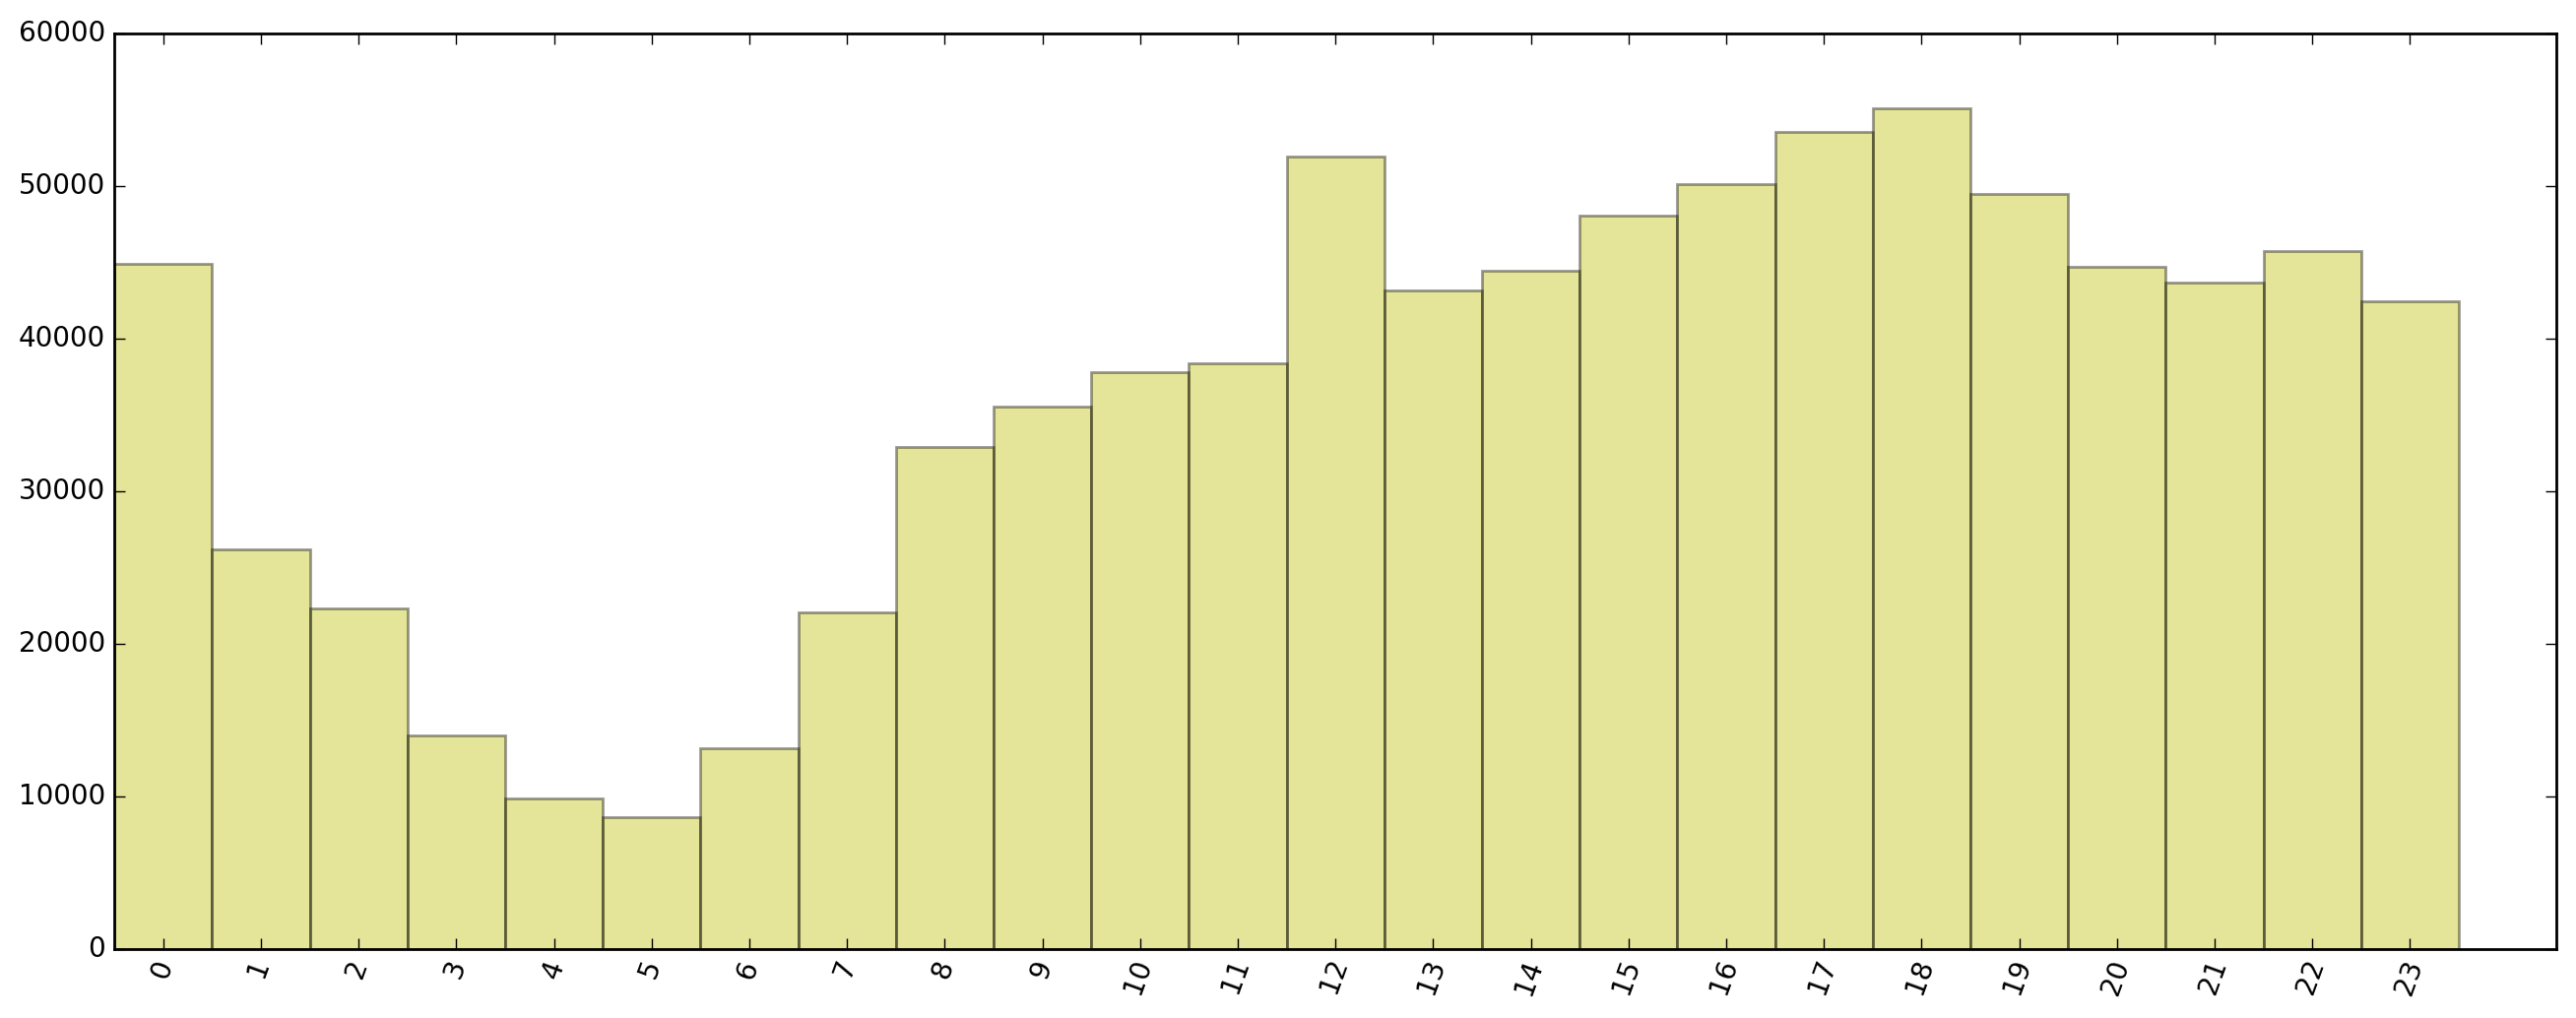
\includegraphics[width=160mm]{hours}
\caption{Cantidad de crímenes por hora.}
\label{fig:hours}
\end{figure}

Fecha es un dato muy útil, algunos features resultantes del procesamiento de ella que vienen inmediatamente a la mente son: la hora, el mes, el año. Pero podemos sacar otros features no menores, por ejemplo deducir si era verano o invierno, si era de día o de noche (inclusive variar el rango de día y de noche según estación, siendo que en invierno oscurece más temprano). Sí observamos el gráfico~\ref{fig:hours}, podemos detectar que entre la una y las siete la cantidad de crímenes baja notablemente y, por lo contrario, hay dos picos a las 12 y a las 18. Todos esos datos se pueden convertir en features para nuestro algoritmo. También podemos sacar el dato sobre el día de semana de la fecha - de esta forma la columna con el día de semana en los sets es, en realidad, reduntante. Si podemos conseguir datos externos, podríamos que fechas fueron feriado.




% subsection deduciendo_features (end)


\subsection{Transformando datos} % (fold)
\label{sub:transformando_datos}

% subsection transformando_datos (end)
El set de datos proporcionado en su estado inicial no sirve para aplicarle los algoritmos típicos de machine learning: contiene datos que un algortimo matemático no tiene una forma de interpretar práctica.

% section tratamiento_de_datos (end)
